\section{RTOS}
Embedded Systeme sind System, welche ein Computer beinhlatet, aber selbst keine sind. Sie bestehen überlicherweise aus Hardware, Mechanik und Software. Embedded Systeme können folgende Eigenschaften besitzen:
\begin{itemize}
	\item \textbf{Reaktive Systeme} interagieren mit ihrer Umbegung.
	\item \textbf{Echtzeit} haben nebst funktionalen Anforderungen auch definierbare zeitliche Anforderungen zu erfüllen.
	\item \textbf{Verlässliche Systeme} sind Systeme, welche hohe Zuverlässichkleitenen erfüllen müssen.
\end{itemize}

Ein \textbf{Deeply Embedded System}, besitzt üblicherweise kein GUI und Betriebssystem. z.b. Hörgerät, ABS-Controllers etc. Bei \textbf{Bare Metal Embedded System} wird auch kein OS verwendet.

\subsection{Definitionen}
Als \textbf{Antwortzeit} (auch turnaround time bezeichnet), setzten sich aus Wartezeit und Bearbeitungszeit zusammen. Ein Echtzeitsystem muss explizit Anforderungen an die Antwortzeit erfüllen. 
\begin{center}
	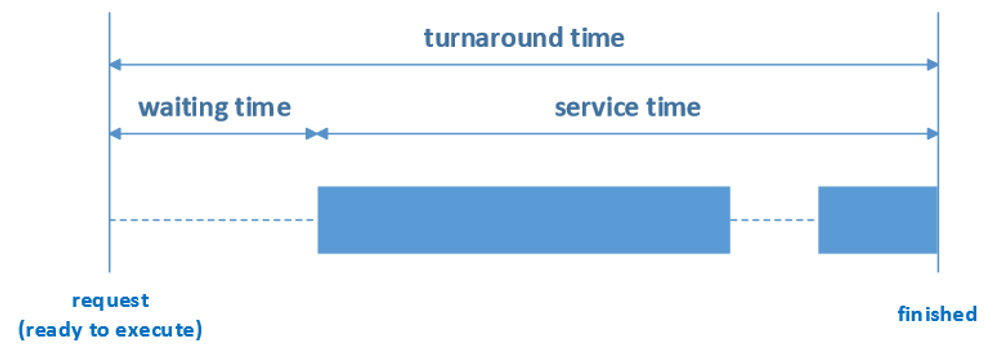
\includegraphics[width=\columnwidth]{Images/zeitdefinition}
\end{center}

Bei \underline{weichen} Echtzeitsyste wird duch Verletzungen der Antwortzeit das System nicht ernsthaft beeinflusst. Hingegen bei \underline{harten} Echtzeitsystem kann ein kompletter Systemausfall entstehen, als drittes gibt es noch die \underline{festen} Systeme, welche durch ein paar 
wenigen verletzungen der Antwortzeiten nicht ernsthaft betroffen sind. Bei vielen jedoch, kann es zu einem komplett Ausfall führen.

\subsection{Scheduler}
Der \textbf{Scheduler} soll sicherstellen, dass Zeiteinschränkungen eingehalten werden. Dazu muss er entscheiden, welcher Task (Job) als nächstes Ausgeführt werden soll. Es gibt diverse Strategien
\begin{enumerate}
	\item FCF: hat Längere Mittlere wartezeit
	\item Round Robin: Fixe Reihenfolge immer wieder ausführen
	\item SIF: Shortest Job First. Nachteil ist, dass längere Tasks verhungern können, dafür wird die mittlere Wartezeit reduziert.
	\item Priority Scheduling: Tiefe Prioritäte Task können verhungern.
\end{enumerate}

\subsubsection{RMS}
Rate Monotonic Scheduling fordert periodische Tasks und static priority preemtive scheduling. Dazu wird für jeden Task die Periode $p_i$ und worst case execution time $e_i$ ermittelt bzw. geschätzt. Die Prioritäten müssen dabei so zugewiesen werden, dass kürzere Perioden höhere Prioritäten erhalten. Jeder Task trägt nun mit der Teilauslastung $u_i = \frac{e_i}{p_i}$ zur Gesammtauslastung $U = \sum_{i}^{}u_i$ bei.

$T_1$ hat die kleinste Periode, und daher die höchste Priorität. Daher wird als erstes $T_1$ und anschliessend die anderen Tasks aufgezeichnet. Man beachte, dass zum Zeitpunkt 4 der am niedrigst priorisierte Task unterbruchen wird. Die Gesammtauslastung beträgt $90\%$ und ist scheduable, weil nach 20 Zyklen wieder von vorne beginnt und 2 noch frei sind.
\begin{center}
	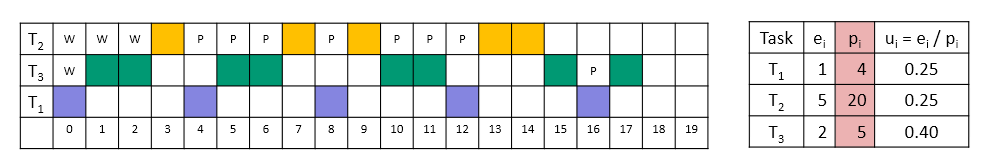
\includegraphics[width=\columnwidth]{Images/rms}
\end{center}

Durch die Formel von Liu und Layland, kann nun abgeschätzt werden, ob es schedulable ist. Wenn die 90\% kleiner als 78\% gewesen wären, dann müsste man die detailierte Aufzeichnung nicht machen.
\begin{center}
	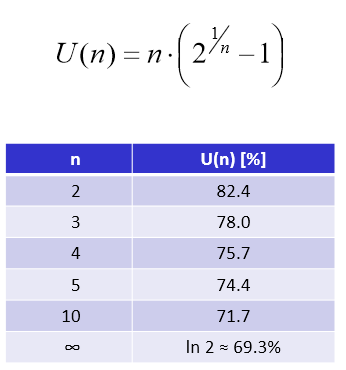
\includegraphics[width=0.5\columnwidth]{Images/rms_def}
\end{center}
